%\title{LaTeX Portrait Poster Template}
%%%%%%%%%%%%%%%%%%%%%%%%%%%%%%%%%%%%%%%%%
% a0poster Portrait Poster
% LaTeX Template
% Version 1.0 (22/06/13)
%
% The a0poster class was created by:
% Gerlinde Kettl and Matthias Weiser (tex@kettl.de)
% 
% This template has been downloaded from:
% http://www.LaTeXTemplates.com
%
% License:
% CC BY-NC-SA 3.0 (http://creativecommons.org/licenses/by-nc-sa/3.0/)
%
%%%%%%%%%%%%%%%%%%%%%%%%%%%%%%%%%%%%%%%%%

%----------------------------------------------------------------------------------------
%	PACKAGES AND OTHER DOCUMENT CONFIGURATIONS
%----------------------------------------------------------------------------------------
\documentclass[a0,portrait]{a0poster}

\usepackage{multicol} % This is so we can have multiple columns of text side-by-side
\columnsep=100pt % This is the amount of white space between the columns in the poster
\columnseprule=3pt % This is the thickness of the black line between the columns in the poster

\usepackage{array}
\newcolumntype{P}[1]{>{\centering\arraybackslash}p{#1}} % for centering columns in table

\usepackage[svgnames]{xcolor} % Specify colors by their 'svgnames', for a full list of all colors available see here: http://www.latextemplates.com/svgnames-colors

%%\usepackage{times} % Use the times font
%\usepackage{palatino} % Uncomment to use the Palatino font
\usepackage{helvet} %basically arial font?
\renewcommand{\familydefault}{\sfdefault}


\usepackage{graphicx} % Required for including images
\graphicspath{{figures/}} % Location of the graphics files
\usepackage{booktabs} % Top and bottom rules for table
\usepackage[font=Large,labelfont=bf]{caption} % Required for specifying captions to tables and figures
\usepackage{amsfonts, amsmath, amsthm, amssymb} % For math fonts, symbols and environments
\usepackage{wrapfig} % Allows wrapping text around tables and figures

\usepackage{subcaption}
%\usepackage[demo]{graphicx}  % remove 'demo' option for your real document

\definecolor{light-gray}{gray}{0.9}
\newcommand{\code}[1]{\colorbox{light-gray}{\texttt{#1}}}

\usepackage{amsmath}
\usepackage[linesnumbered,ruled]{algorithm2e}

\usepackage[export]{adjustbox}

\usepackage{array}

\begin{document}

%----------------------------------------------------------------------------------------
%	POSTER HEADER 
%----------------------------------------------------------------------------------------

% The header is divided into two boxes:
% The first is 75% wide and houses the title, subtitle, names, university/organization and contact information
% The second is 25% wide and houses a logo for your university/organization or a photo of you
% The widths of these boxes can be easily edited to accommodate your content as you see fit


\begin{minipage}[b]{0.80\linewidth}
\veryHuge \color{NavyBlue} \textbf{(Group) Iterative Hard Thresholding for GLM in Statistical Genetics}\\
\\
\\
\\
\color{Black} % Title
%\Huge\textit{In the Julia programming language }\\[2cm] % Subtitle
\noindent \huge \textbf{Benjamin Chu, Kevin Keys, Janet Sinsheimer, and Kenneth Lange}\\[0.5cm] % Author(s)
\huge Dept. of Biomathematics, University of California, Los Angeles, CA, USA\\[0.4cm]
\normalsize 
Contacts: \texttt{biona001@ucla.edu, kevin.keys@ucsf.edu, jsinshei@ucla.edu,  klange@ucla.edu} \\
Git Repository: \texttt{https://github.com/biona001/IHT.jl} \\
\end{minipage}
%
\begin{minipage}[b]{0.25\linewidth}
\centering
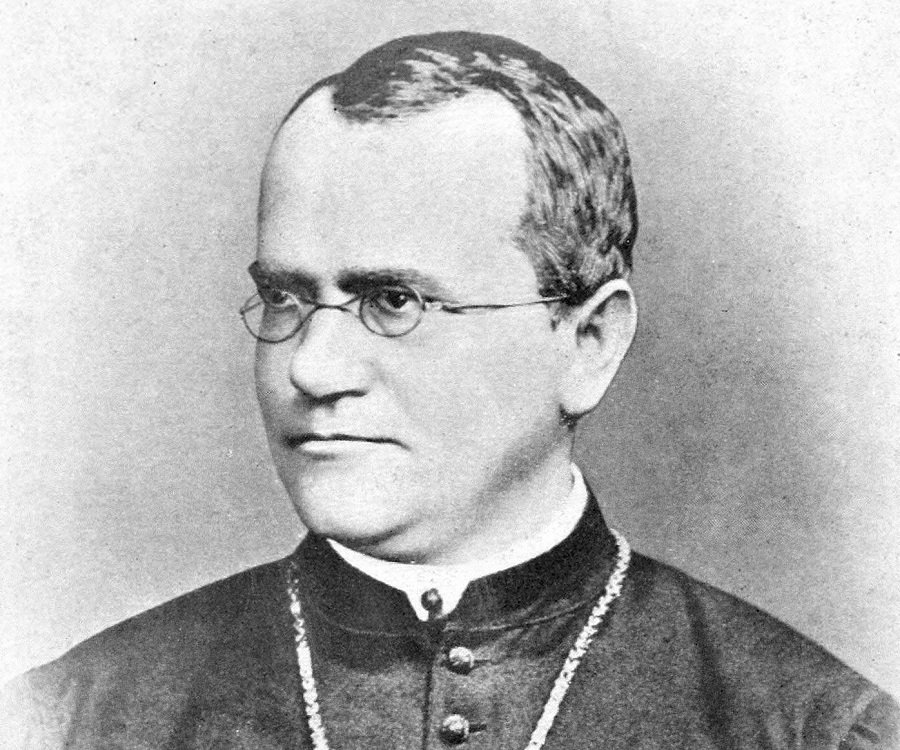
\includegraphics[width=12cm]{figures/gregor-mendel-3.jpg}

\includegraphics[width=15cm]{figures/ucla-std-blu-cmyk.jpg}
\end{minipage}

%\vspace{1cm} % A bit of extra whitespace between the header and poster content

%----------------------------------------------------------------------------------------

\begin{multicols}{2} % This is how many columns your poster will be broken into, a portrait poster is generally split into 2 columns

\color{Navy} % Navy color for the abstract
\section*{Background:}

\color{Black} % Navy color for the abstract

\large

\raggedright
Individual variations in the DNA sequence are termed \textbf{single nucleotide polymorphisms} (SNPs), and they can be identified experimentally via \textbf{Genome Wide Association Studies} (GWAS). These studies aim to answer one main question:

\vspace{1cm}
\centering \Large \textbf{Q: Which genetic variants explain variations in a trait?}

\vspace{1cm}

\raggedright \large

\begin{center}
\color{Black} \footnotesize Picture references: CONVERGE consortium, \textit{Nature} (2015) and Balding et al. \textit{Nature Review Genetics} (2006).
\end{center}

\begin{center}
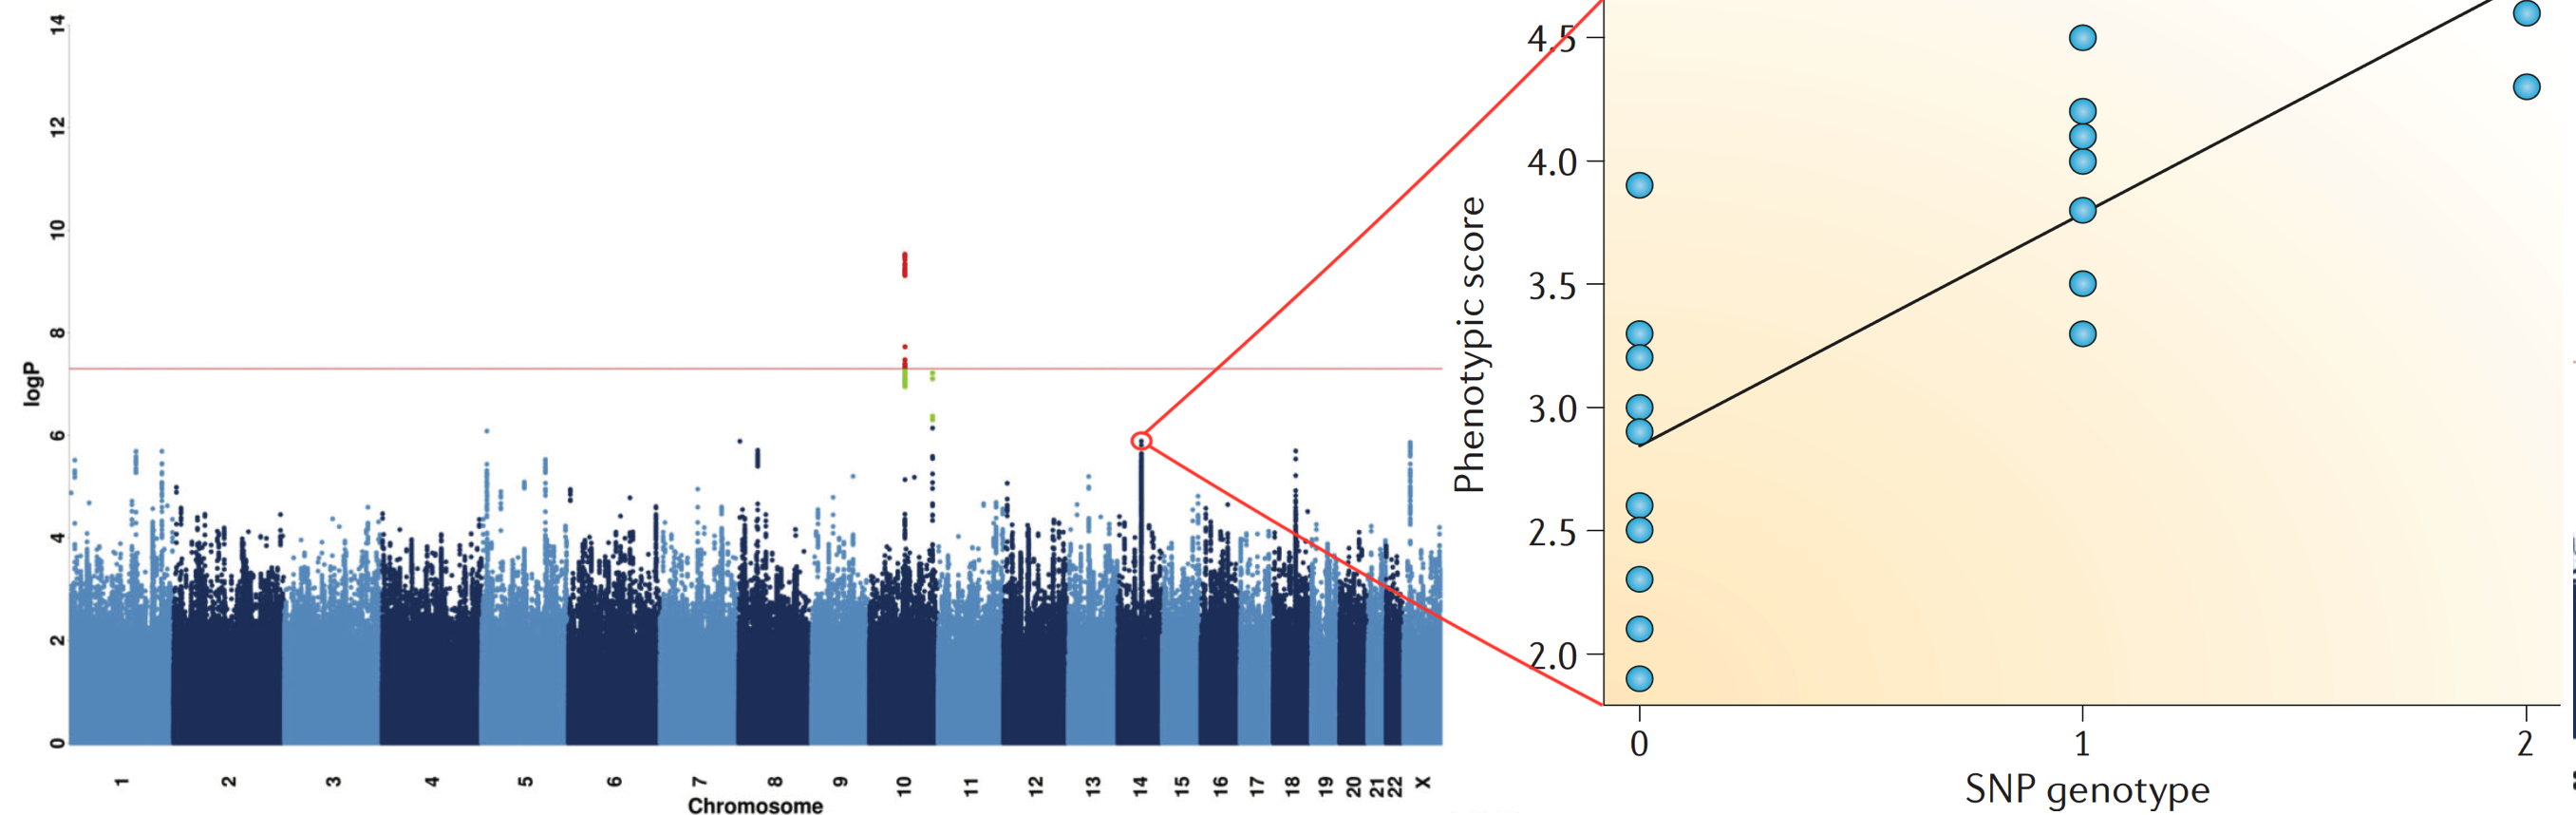
\includegraphics[width=1.0\linewidth]{intro_ver2.png}
\captionof{figure}{\color{Green} \textbf{Traditional analysis assigns a p-value for each SNP based on a linear regression that test if slope $\neq$ 0}}
\end{center}

\color{Navy} % Navy color for the abstract
\section*{Problems with Traditional Analysis (See Figure 1):}
\color{black}

\large
\begin{itemize}
	\item Individual SNP association testing ignores joint effects of multiple SNPs and suffers high multiple testing burden. \textbf{\color{Green} Q: What is the best multivariate model selection method to use? }
	\item GWAS dataset sizes are growing rapidly (100+ GB). \textbf{\color{Green} Q: How to analyze them efficiently? } \color{black}
	\item SNPs are sometimes \textbf{rare} with \textbf{small effect size}. \color{Green} \textbf{Q: How to separate \textit{weak signals} from \textit{noise}}?  \color{black}
\end{itemize}

\color{Navy} % Navy color for the abstract

%\section*{Intuition: IHT iterates between gradient descent and projection}

%\begin{center}
%\vspace{1cm}
%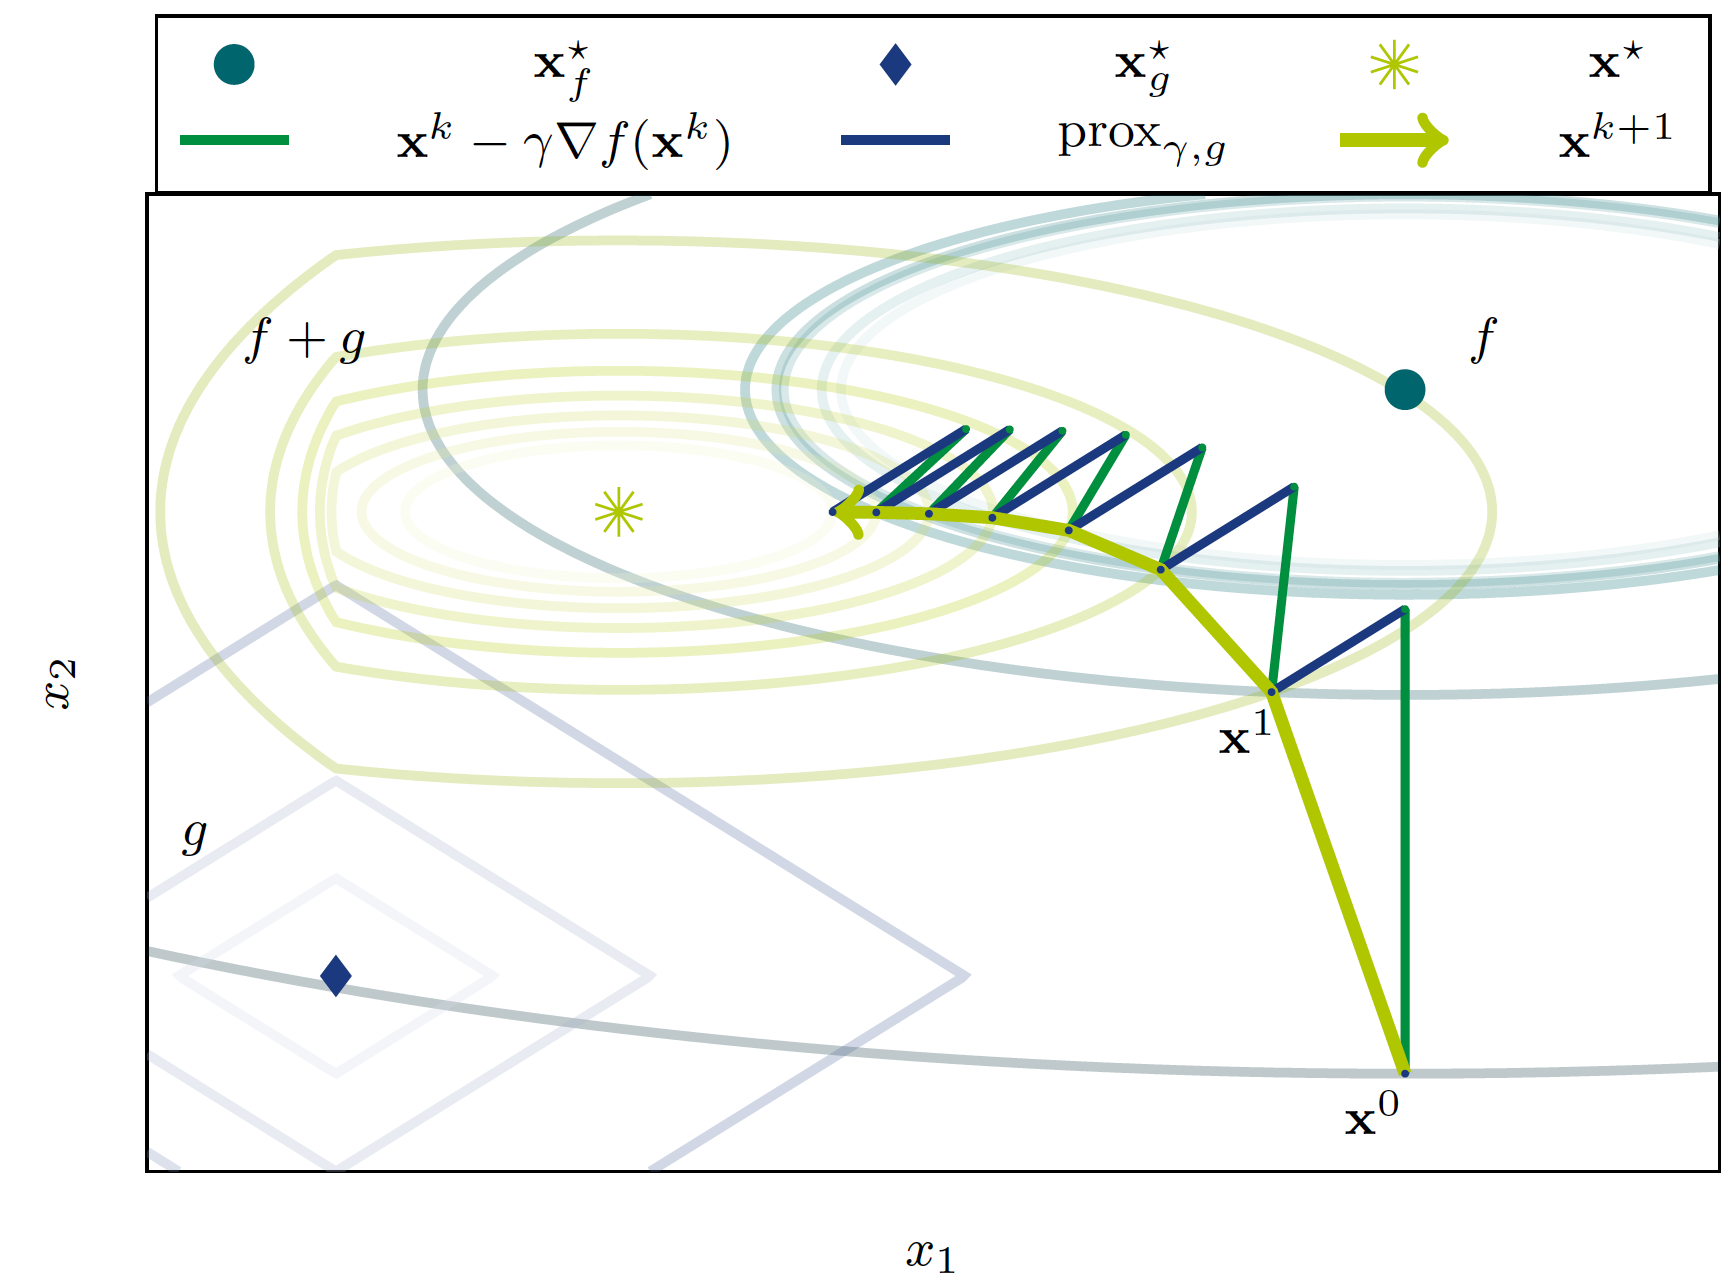
\includegraphics[width=0.5\linewidth]{figures/IHT_graph.png}

%\color{Black} \footnotesize Antonello, Niccolò, et al. "Proximal Gradient Algorithms: Applications in Signal Processing." arXiv preprint arXiv:1803.01621 (2018).
%\end{center}

\color{Navy} % Navy color for the abstract

\section*{IHT: $\ell_0$ Sparsity without Shrinkage}

\color{Black} % SaddleBrown color for the introduction

\begin{center}
%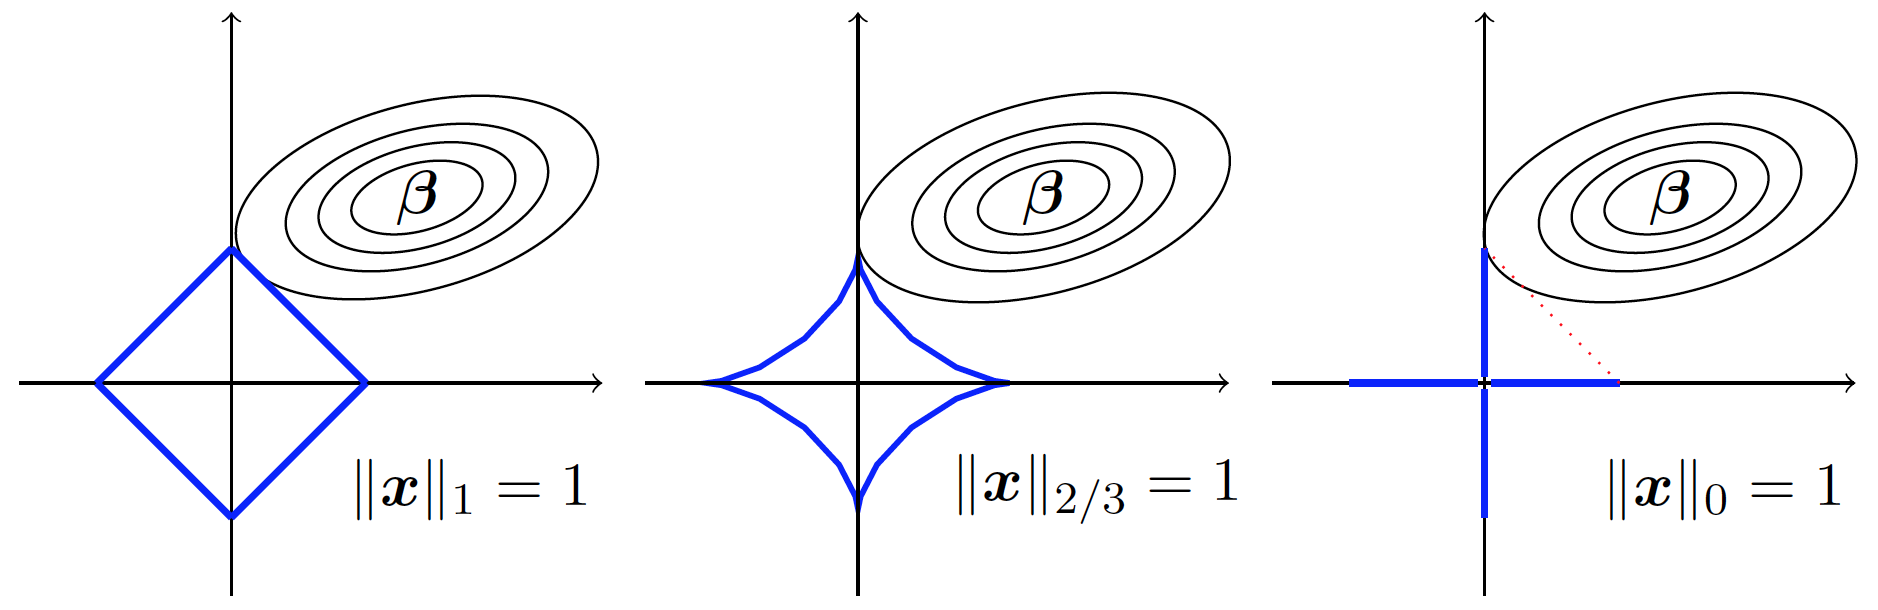
\includegraphics[width=0.7\linewidth]{sparsity.png}
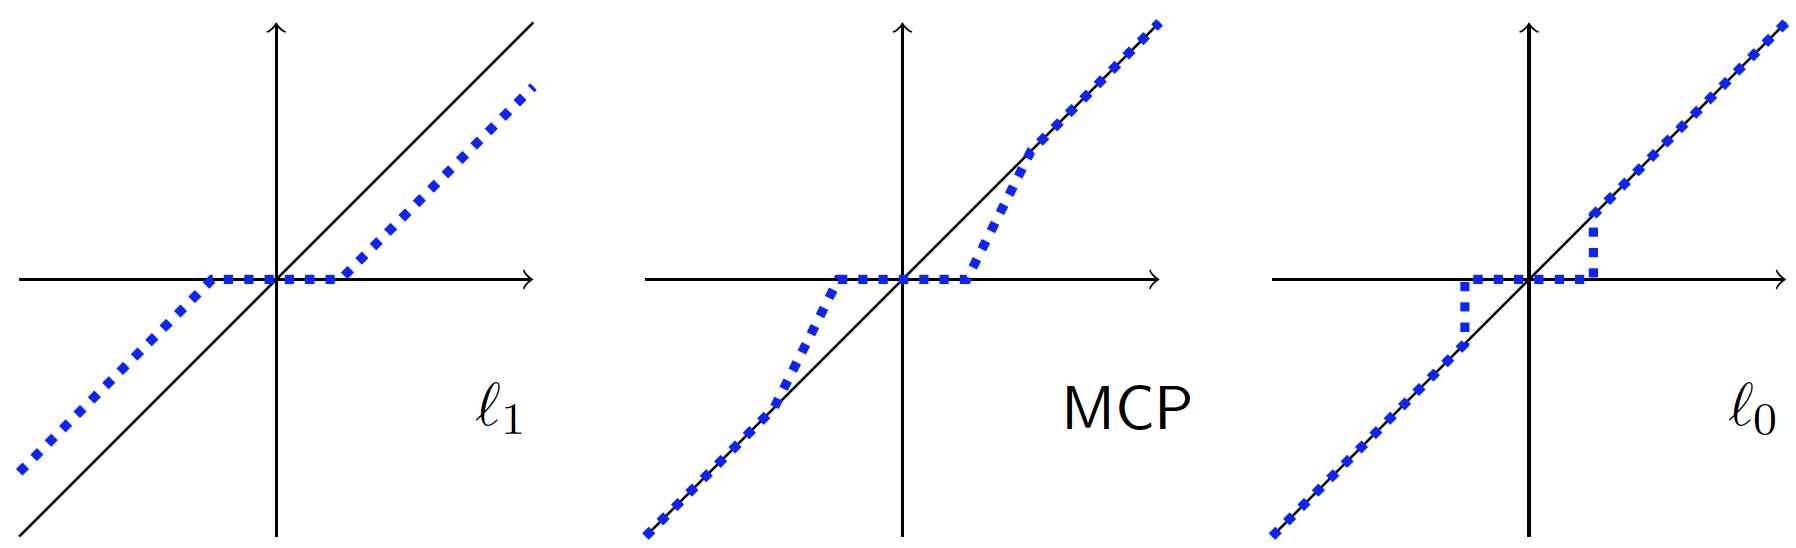
\includegraphics[width=0.7\linewidth]{shrinkage.png}
\captionof{figure}{\color{Green} \textbf{Biological meaning = IHT potentially captures variants with small effect size}}
\end{center}

%----------------------------------------------------------------------------------------
%	Math
%----------------------------------------------------------------------------------------

\color{Navy} 
\section*{Using IHT to find GLM coefficients via MLE}

\color{Black}

Iterative hard-thresholding (IHT) performs \textit{feature selection} for $\mathbf{X}^{n \times p}$ when $p \gg n$. First we expand the framework of IHT to any generalized linear model. Then we modified the thresholding operator to enforce sparsity on the group-level as well as within groups. 

\subsection*{(Group) IHT algorithm}

 Let $L(\beta)$ be the loglikelihood, $\mathbf{v} = -\nabla L(\beta)$ the negative score (gradient), $J(\beta)$ the expected (Fisher) information matrix, and $S_{R, k}$ a predictor set with at most $R$ active groups and $k$ active predictors per group. We maximize the loglikelihood iteratively via:

\begin{align*}
	\beta^{(n+1)} = \mathcal{P}_{S_{R, k}}\left( \beta^{(n)} + s\mathbf{v} \right)
\end{align*}
\begin{align*}
	s = \frac{||\mathbf{v}||^2_2}{\mathbf{v}^TJ(\beta^{(n)})\mathbf{v}} = \text{ step size,} \quad \mathcal{P}_{S_{R, k}}(\mathbf{v}) \text{ projects } \mathbf{v} \text{ to } S_{R, k}
\end{align*}

\vspace{1cm}

%\begin{algorithm*}[H]
%    \SetKwInOut{Input}{Input}
%    \SetKwInOut{Output}{Output}
%
%    \Input{genotype matrix $\mathbf{X}$, response vector $\mathbf{y}$, membership indicator vector $\mathbf{G}$, scalars $R, k$}
%    \Output{$\beta$ with at most $R$ active groups and $k$ active predictors per group}
%    \textbf{Initialize:} $\beta \equiv \mathbf{0}.$\\
%    
%    \While{not converged}
%      {
%        \textbf{Gradient step:} $\tilde{\beta} = \beta^n + sv$\\
%        \textbf{Projection:} $\beta^{n+1} = \mathcal{P}_{J, k}(\tilde{\beta})$\\
%        \textbf{(Optional) Debiasing}: $\beta^{n+1} = \arg \min f(\beta^{n+1})$ such that $supp(\beta^{n+1})$ satisfies constraints described in (1)
%      }
%    \caption{\large (Group) Iterative hard-thresholding}
%\end{algorithm*}

%----------------------------------------------------------------------------------------
%	RESULTS 
%----------------------------------------------------------------------------------------

\color{Navy}
\section*{Results}
\color{Black}

\begin{center}
\begin{tabular}{ |P{6cm}||P{6cm}|P{6cm}|P{6cm}|  }
 \hline
 \multicolumn{4}{|c|}{IHT Reconstruction Results} \\
 \hline
 $\beta_{true}$ & $\beta_{\text{normal}}$ & $\beta_{\text{logistic}}$ & $\beta_{\text{poisson}}$\\
 \hline
2.15035 & 2.15076 & 2.31195 & 2.15246 \\
1.42043 & 1.41833 & 1.51125 & 1.42261\\
-1.28871 & -1.28929 & -1.36258 & -1.2846 \\ 
-1.04068 & -1.04139 & -1.07631 & -1.04235\\ 
0.546087 & 0.548324 & 0.700991 & 0.545524\\
0.360115 & 0.360985 & 0.417808 & 0.358854 \\
0.331856 & 0.335209 & 0.388734 & 0.329764 \\
0.279001 & 0.278694 & 0.304497 & 0.279266 \\
0.103375 & 0.103152 & \text{Not Found} & 0.100905 \\
0.0344145 & 0.0363563 & \text{Not Found} & 0.0329963\\
 \hline
\end{tabular}\par \bigskip
\Large \color{Green} Simulated result with $n = 5000$ subjects and $p = 100,000$ SNPs. $\beta_{true} \sim N(0,1)$ and responses were simulated via canonical link. 
\end{center}

\begin{center}\vspace{1cm}
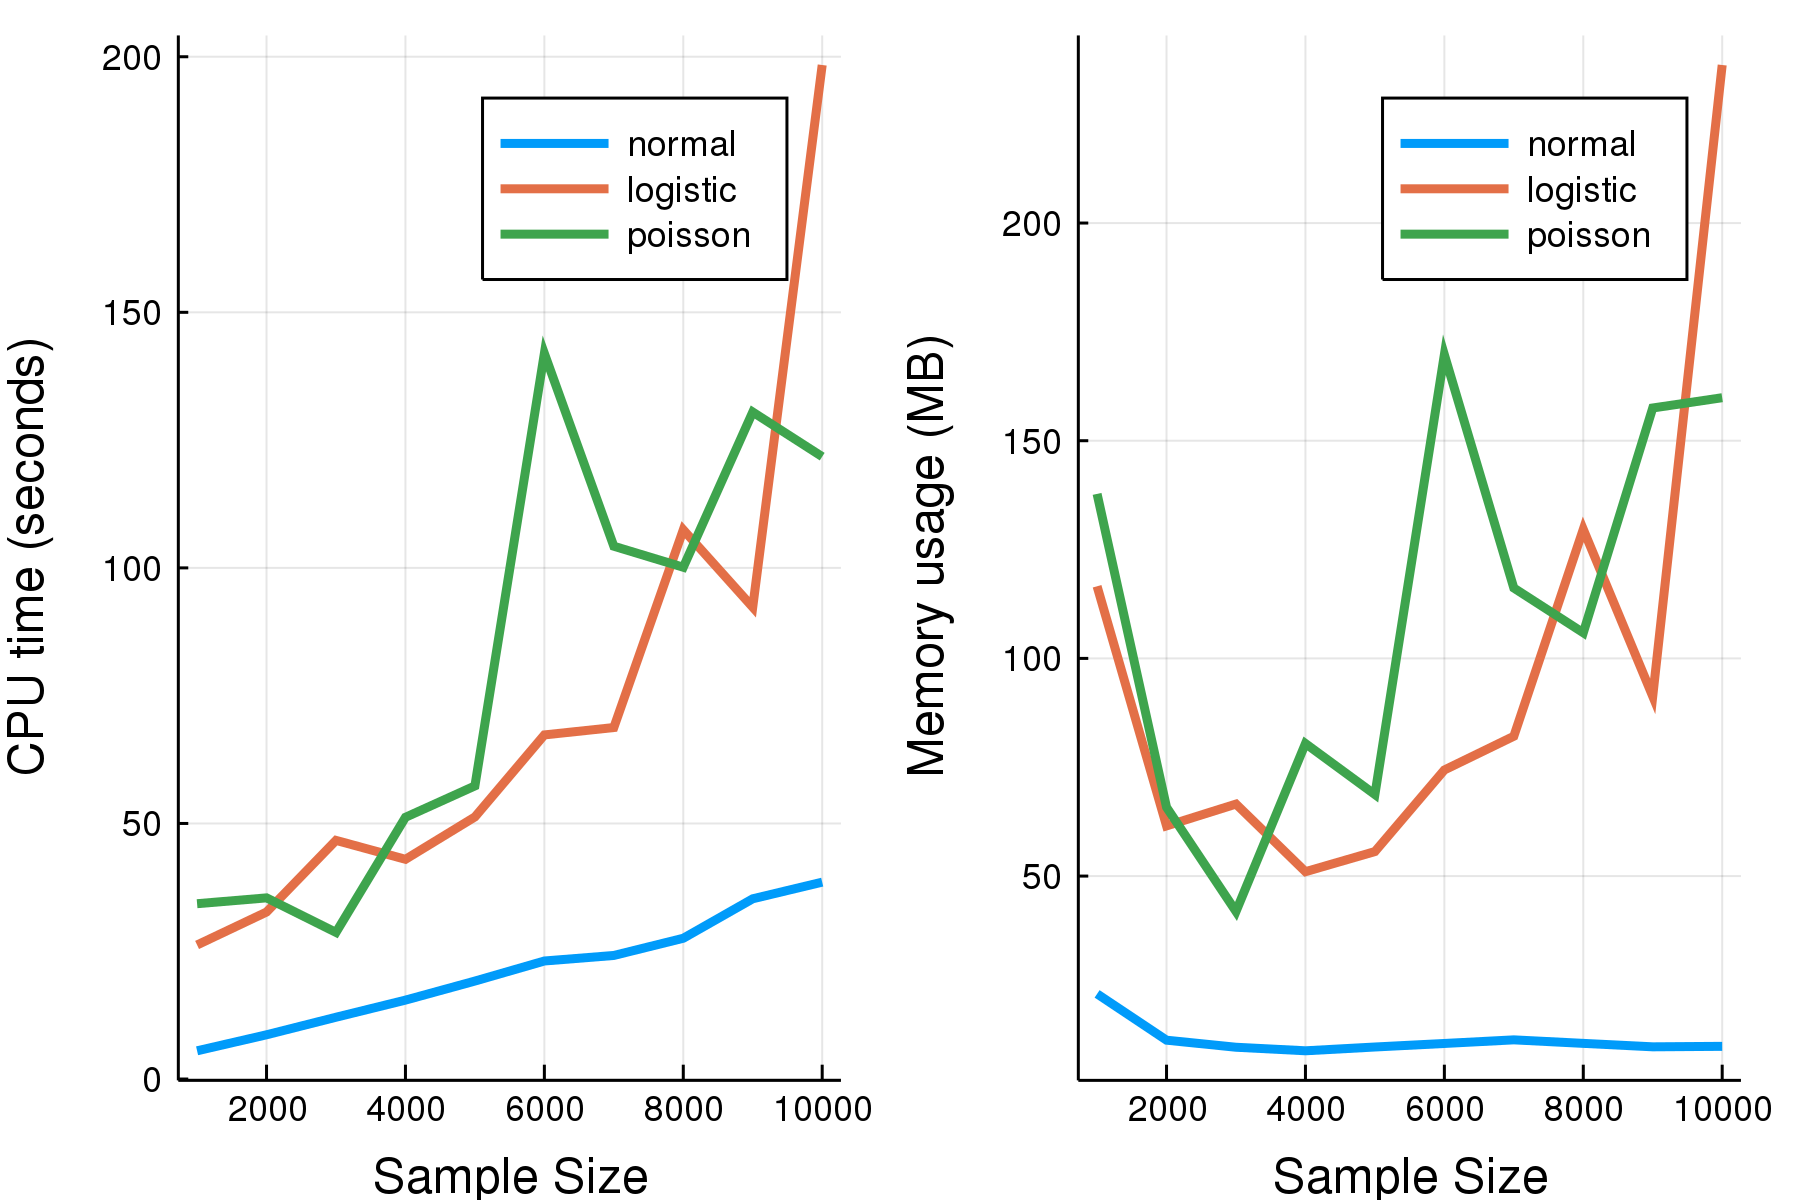
\includegraphics[width=0.9\linewidth]{figures/speed_mem_benchmark.png}
\captionof{figure}{\color{Green} \textbf{Speed and memory benchmark on 100000 SNPs}}
\end{center}\vspace{1cm}

\begin{center}\vspace{1cm}
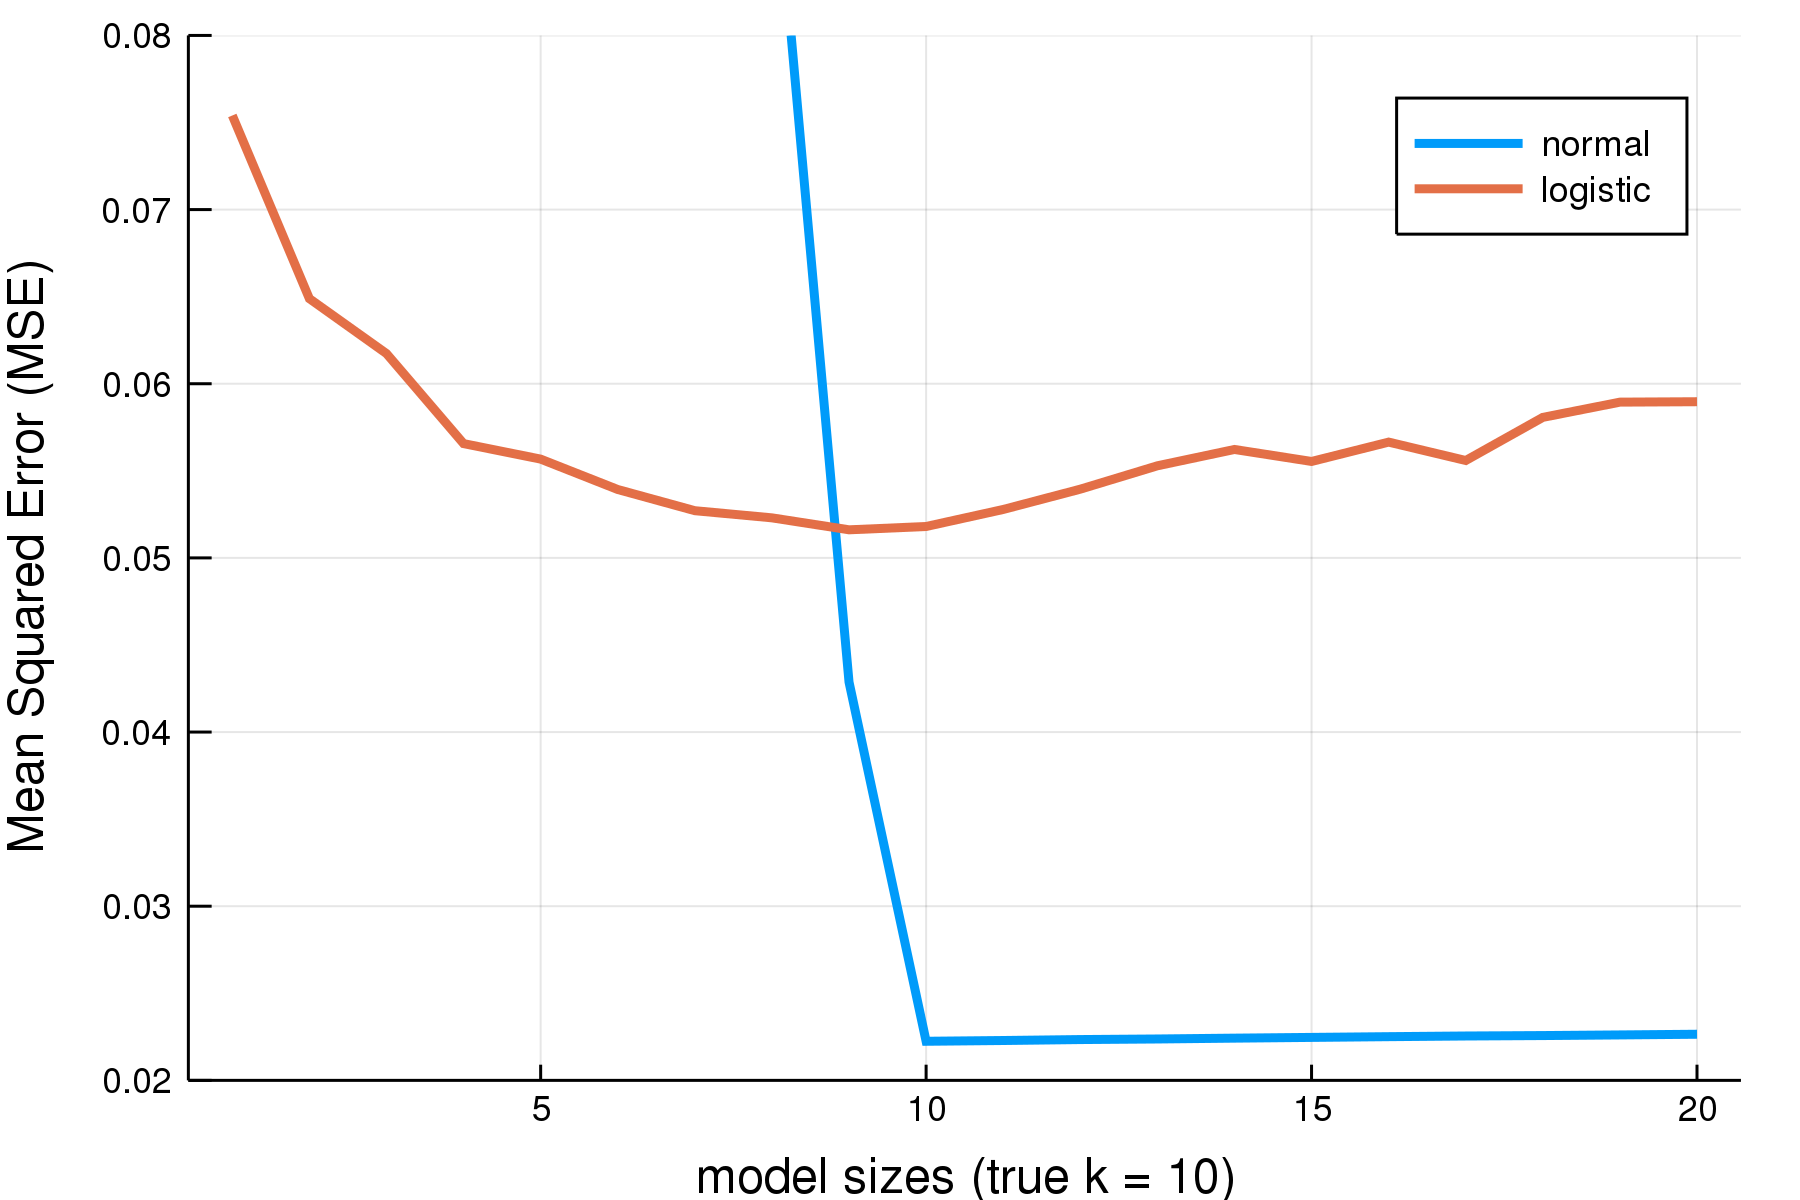
\includegraphics[width=0.7\linewidth]{figures/mse.png}
\captionof{figure}{\color{Green} Cross-validation finds $k_{\text{normal}}^\text{estimate} = 10$ and $k_{\text{logistic}}^\text{estimate} = 9$}
\end{center} 

\color{Navy}
\section*{Summary of Results}
\color{Black}

\begin{itemize}
	\item We applied IHT to perform multivariate model selection on genetics data.
	\item IHT can recover small effect sizes without shrinkage. 
	\item Computational time increases linearly with data size. 
	\item Memory usage remains relatively constant with data size.
	\item Cross Validation works well to determine the true model size $k_{\text{true}}$. 
\end{itemize}

%Figure 2 below compares matrix-vector multiplication speed of BLAS and SnpArrays. For big enough matrices, SnpArrays is faster:
%\begin{center}\vspace{1cm}
%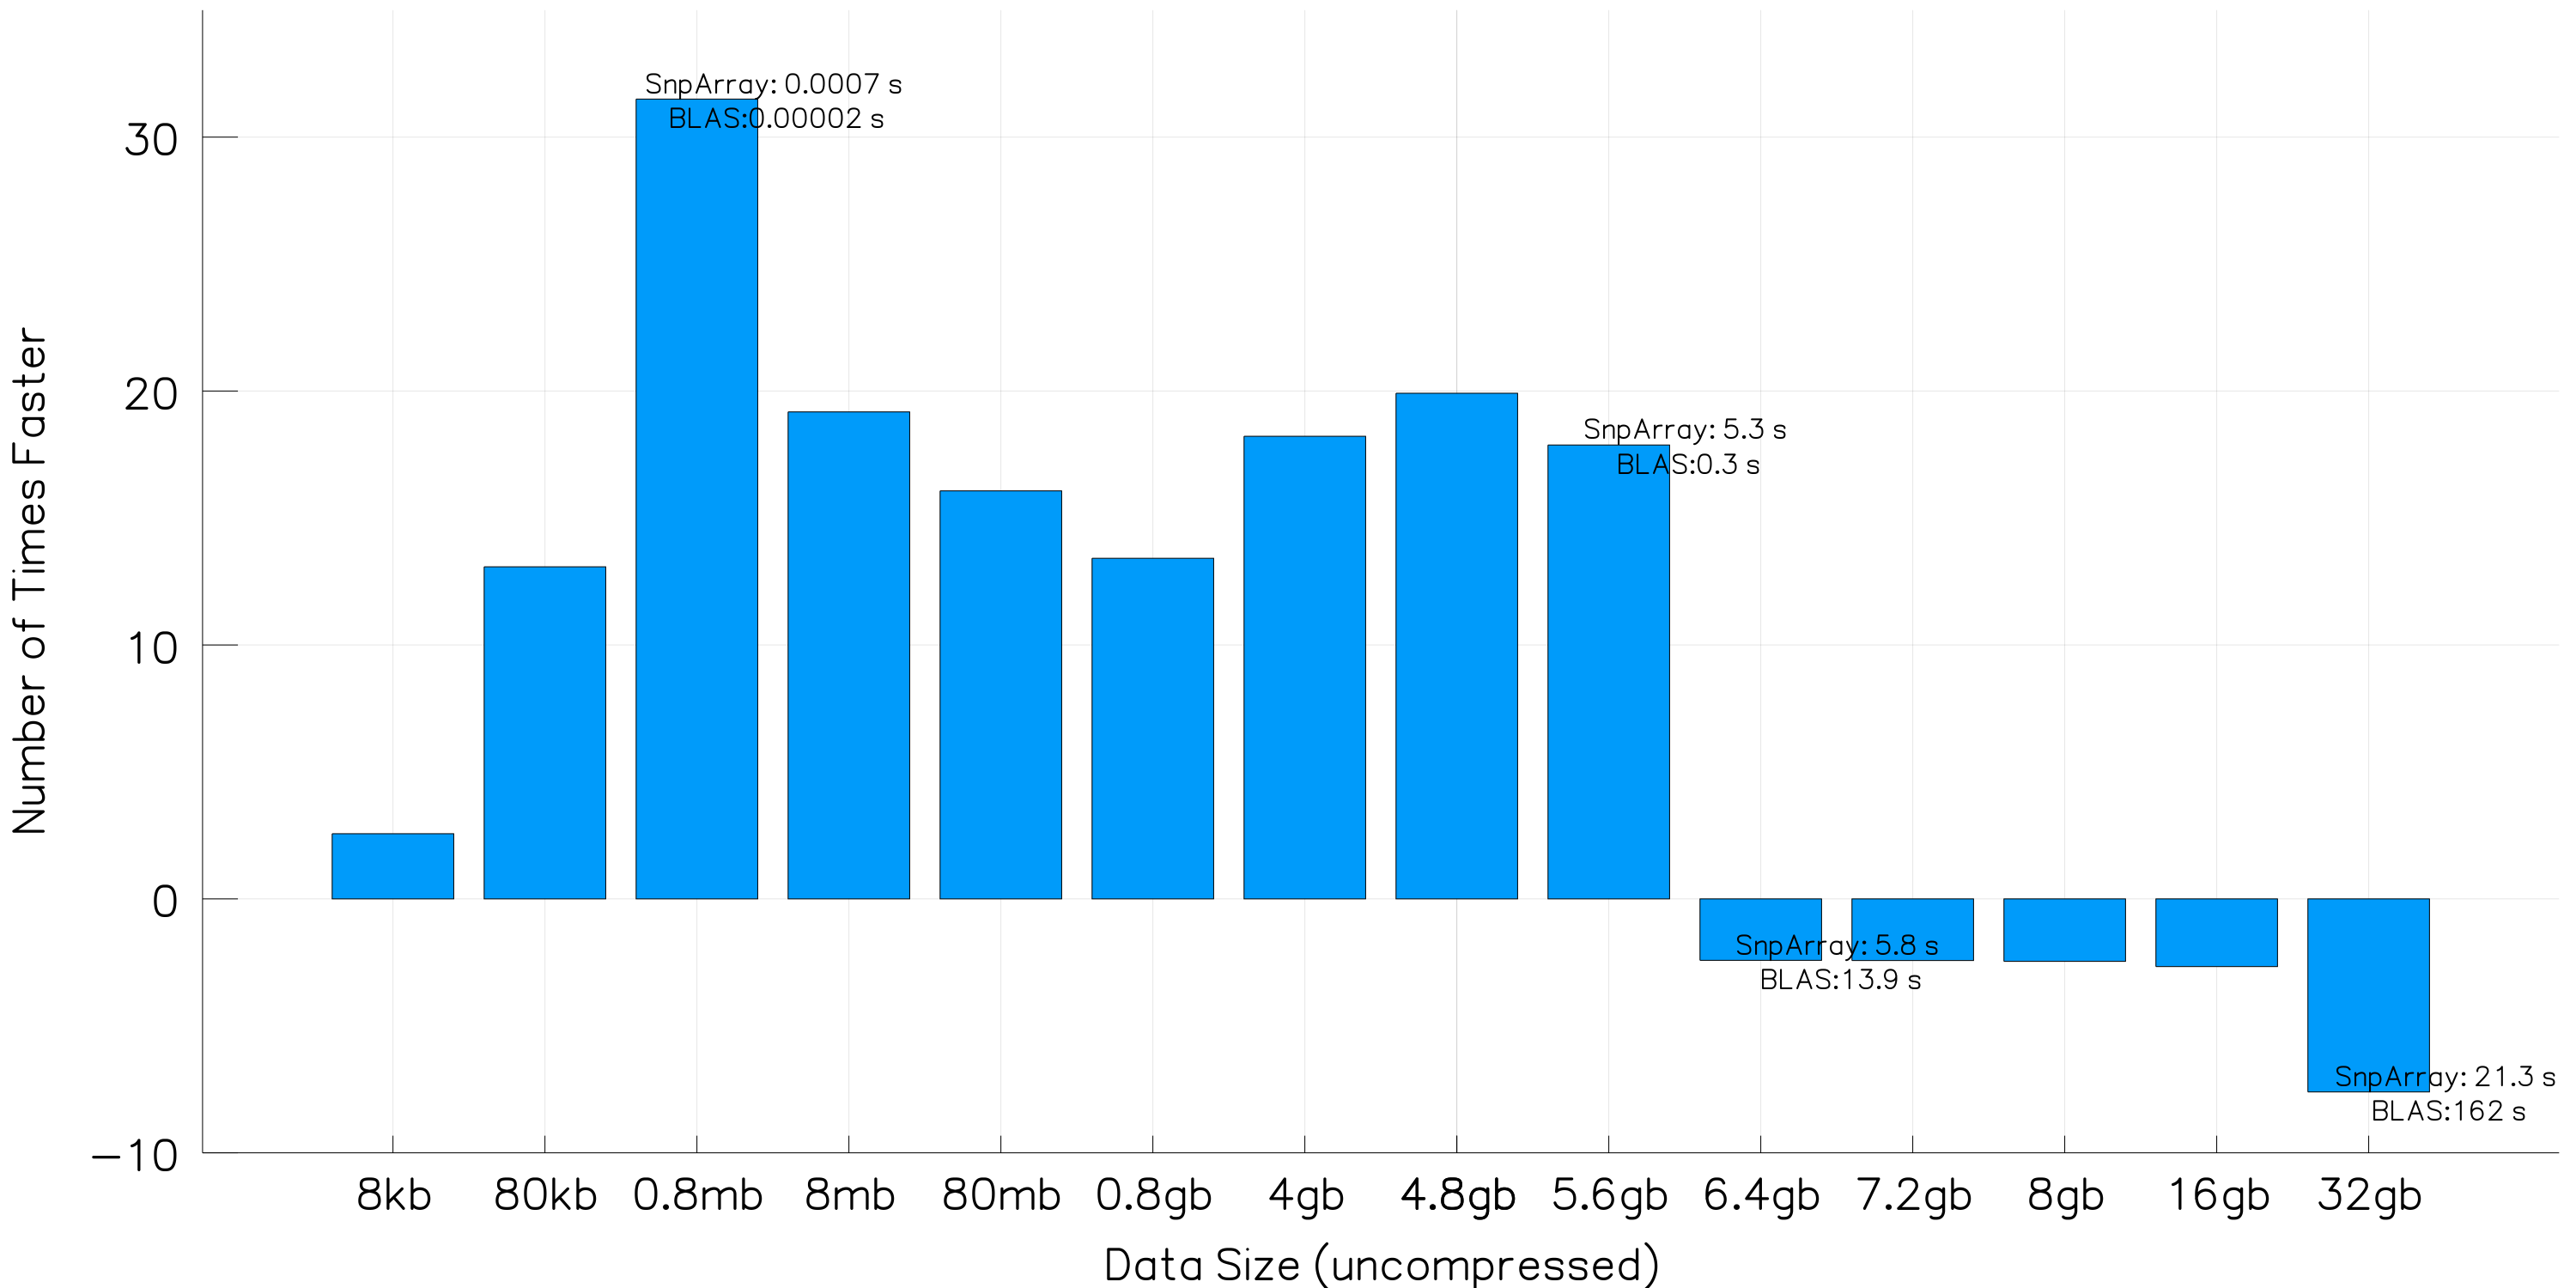
\includegraphics[width=0.9\linewidth]{figures/compare.png}
%\captionof{figure}{\color{Green} \textbf{Linear Algebra in SnpArrays is faster than BLAS for Large Matrices}}
%\end{center}\vspace{1cm}


%----------------------------------------------------------------------------------------
%	ACKNOWLEDGEMENTS
%----------------------------------------------------------------------------------------
\color{Navy}
\section*{Acknowledgements}
\color{Black}
\begin{itemize}
\item This research was supported by NIH Training Grant in Genomic Analysis and Interpretation T32HG002536
\item This research was supported by Google Summer of Code 2018 with NumFOCUS, Julia cohort 
\end{itemize}
%----------------------------------------------------------------------------------------

\end{multicols}
\end{document}